%%%%%%%%%%%%%%%%%%%%%%%%%%%%%%%%%%%%%%%%%%%%%%%%%%%%%%%%%%%%%%%%%%%%%%%%%%%
%
% Plantilla para un artículo en LaTeX en español.
%
%%%%%%%%%%%%%%%%%%%%%%%%%%%%%%%%%%%%%%%%%%%%%%%%%%%%%%%%%%%%%%%%%%%%%%%%%%%

% Qué tipo de documento estamos por comenzar:
\documentclass[a4paper]{article}
% Esto es para que el LaTeX sepa que el texto está en español:
\usepackage[spanish]{babel}
\selectlanguage{spanish}
% Esto es para poder escribir acentos directamente:
\usepackage[utf8]{inputenc}
\usepackage[T1]{fontenc}



%% Asigna un tamaño a la hoja y los márgenes
\usepackage[a4paper,top=3cm,bottom=2cm,left=3cm,right=3cm,marginparwidth=1.75cm]{geometry}

%% Paquetes de la AMS
\usepackage{amsmath, amsthm, amsfonts}
%% Para añadir archivos con extensión pdf, jpg, png or tif
\usepackage{graphicx}
\usepackage[colorinlistoftodos]{todonotes}
\usepackage[colorlinks=true, allcolors=blue]{hyperref}

%% Primero escribimos el título
\title{Un algoritmo de dos fases para reconocer las actividades humanas en el contexto de la Industria 4. 0 y los procesos impulsados por el hombre}
\author{Borja Bordel$^1$, Ramón Alcarria$^1$, Diego Sánchez-de-Rivera$^1$\\
  \small $^1$Universidad Politécnica de Madrid, Madrid, España\\
  \small bbordel@dit.upm.es, ramon.alcarria@upm.es, diegosanchez@dit.upm.es\\
  \date{}
}

%% Después del "preámbulo", podemos empezar el documento

\begin{document}
%% Hay que decirle que incluya el título en el documento
\maketitle

%% Aquí podemos añadir un resumen del trabajo (o del artículo en su caso) 
\begin{abstract}
Esta es una plantilla simple para crear un articulo \LaTeX en español, con algunos comandos que se usarán frecuentemente para hacer tareas de la licenciatura en Física.
\end{abstract}

%% Iniciamos "secciones" que servirán como subtítulos
%% Nota que hay otra manera de añadir acentos
\section{Introducci\'on}

¡Tu introducción va aquí! A continuación, se enumeran algunos ejemplos de comandos y funciones de uso común para ayudarte a comenzar.

\section{Algunos ejempllos para comenzar}

\subsection{¿Cómo incluir figuras?}

Primero tienes que cargar el archivo de imagen desde su computadora usando el enlace de carga del menú del proyecto. Luego usando el comando 'includegraphics' podrás incluirlo en el documento. Con el entorno de figura y el comando de título podrás agregar un número y un título a la figura. Mira el código de la Figura \ref{fig:tesla} en esta sección para ver un ejemplo.

\begin{figure}
\centering
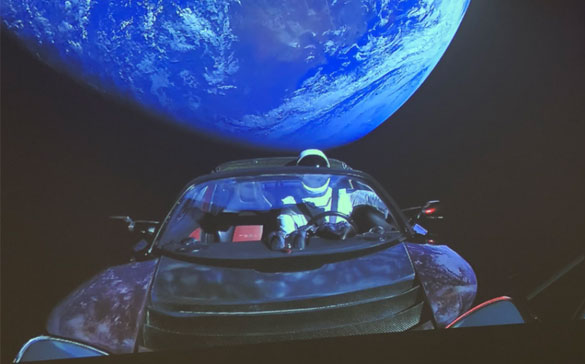
\includegraphics[width=0.5\textwidth]{tesla.jpg}
\caption{\label{fig:tesla}Esta imagen se añadió en el menú Project.}
\end{figure}


\subsection{¿Cómo añadir comentarios?}
% * <stephmigoni@gmail.com> 2018-02-08T19:23:33.559Z:
% 
% Esto es un comentario de prueba
% 
% 

Puedes añadir comentarios en el ícono + del menú de arriba.

Para responder a un comentario, simplemente da click en Reply en Rich Text.

También pueden añadirse comentarios en el margen del pdf compilado con el comando todo \todo{¡Comment en el margen!}, como se muestra en el ejemplo de la derecha. También puedes añadirlos dentro del texto:

\todo[inline, color=green!40]{Este es un comentario dentro del texto.}

\subsection{¿Cómo añadir tablas en mi \TeX?}

Usa los comandos table y tabular para iniciar una tabla simple --- mira la tabla~\ref{tab:tabla ejemplo}, como ejemplo. 

\begin{table}
\centering
\begin{tabular}{l c r} 
%nùmero de columnas: 3
l para left & c para centro & r para derecha \\ \hline
Ejemplo & Centrado & Alineado a la\\
Izquierda & 13 & Derecha
\end{tabular}
\caption{\label{tab:tabla ejemplo}Una simple tabla.}
\end{table}

\subsection{¿Cómo escribir (expresiones) Matemáticas?}

\LaTeX{} es buenísimo para escribir ecuaciones. Para escribir variables o ecuaciones dentro del texto lo podemos poner entre signos de pesos y luego podemos seguir escribiendo, esto funciona si queremos escribir un símbolo como $\nabla$, $\pi$, $\beta$, $\Omega$, $\aleph$, etc.
\begin{equation}
\sum_{n=0}^\infty \frac{x^n}{n!}=e^x
\end{equation}
\begin{equation}
\int_{0}^{1}dx=1
\end{equation}
\begin{equation}
e^{i\pi}+1=0
\end{equation}
Si queremos citar al gran Maxwell, lo podemos hacer como en la ecuación \ref{eq:Maxwell}:
\begin{equation}
\nabla\times\mathbf{E}+\frac{\partial\mathbf{B}}{\partial t}=0\label{eq:Maxwell}
\end{equation}

A continuación se añade un ejemplo de un desarrollo:
Con este preámbulo llevamos a cabo la siguiente transformación de los operadores $\hat{a}_{\ell}$

\begin{equation}
\hat{b}_{m}^{\dagger}=\sum_{\ell}U_{m}^{\ell}\hat{a}_{\ell}^{\dagger}
\end{equation}

donde $U_{m}^{\ell}$ es un elemento de la matriz unitaria $\mathbf{U}$.

Calculamos ahora su hermitiano conjugado
\begin{align}
\hat{b}_{m} & =\left(\sum_{\ell}U_{m}^{\ell}\hat{a}_{\ell}^{\dagger}\right)^{\dagger}\label{eq:bm}\\
 & =\sum_{\ell}\left(U_{m}^{\ell}\hat{a}_{\ell}^{\dagger}\right)^{\dagger}\nonumber \\
 & =\sum_{\ell}\left(U_{m}^{\ell}\right)^{*}\hat{a}_{\ell}\nonumber \\
 & =\sum_{\ell}\left(U^{-1}\right)_{\ell}^{m}\hat{a}_{\ell},\label{eq:bSubM}
\end{align}

Ahora, para añadir una matriz:

$$
\begin{matrix} 
a & b \\
c & d 
\end{matrix}
\quad
\begin{pmatrix} 
a & b \\
c & d 
\end{pmatrix}
\quad
\begin{bmatrix} 
a & b \\
c & d 
\end{bmatrix}
\quad
\begin{vmatrix} 
a & b \\
c & d 
\end{vmatrix}
\quad
\begin{Vmatrix} 
a & b \\
c & d 
\end{Vmatrix}
$$
%% Por ejemplo, el triple producto escalar:
\begin{equation}
\vec{A}\cdot(\vec{B}\times\vec{C})=\begin{vmatrix}
A_x&A_y&A_z\\
B_x&B_y&B_z\\
C_x&C_y&C_z\\
\end{vmatrix}
\end{equation}

\subsection{¿Cómo añadir listas?}

Puedes añadir listas con numeración automática \dots

\begin{enumerate}
\item Como esta,
\item y como esta.
\end{enumerate}
\dots o con puntitos \dots
\begin{itemize}
\item Como este,
\item y como este.
\end{itemize}

\subsection{¿Cómo añado una lista de Citas y Referencias?}

Puedes subir un archivo \verb|.bib| que contenga todas tus referencias en estilo BibTeX (puedes buscar la bibliografía de un libro en google añadiendo 'bibtex' al final), creado con JabRef. Luego podrás hacer citas así: \cite{Griffiths:1492149}.

Puedes encontrar un \href{https://www.overleaf.com/help/97-how-to-include-a-bibliography-using-bibtex}{video tutorial aquí} para aprender más acerca de BibTeX.

Espero que esta charla haya sido de tu ayuda. Puedes acceder a Overleaf en el siguiente link: \url{https://www.overleaf.com/}!

\bibliographystyle{abbrv}
\bibliography{sample}

\end{document}